\documentclass[french]{book}
\usepackage[utf8x]{inputenc}
\usepackage[T1]{fontenc}
\usepackage{babel}
\usepackage{lmodern}
\usepackage[top=2cm,bottom=2cm,left=3cm,right=3cm]{geometry}
\usepackage{microtype}
\usepackage{mathtools, amssymb, amsthm}
\usepackage{dsfont}
\usepackage{mdframed}
\usepackage{hyperref}
\usepackage{graphicx}
\usepackage{float}
\usepackage{xcolor}
\usepackage{mathrsfs}
\usepackage{wrapfig}
\usepackage{stmaryrd}
\usepackage{framed}


\newtheorem{prototheorem}{Théorème}[section]
\newenvironment{thm}
   {\colorlet{shadecolor}{red!7}\begin{shaded}\begin{prototheorem}}
   {\end{prototheorem}\end{shaded}}

\newtheorem{protocorollary}[prototheorem]{Corollaire}
\newenvironment{corollary}
    {\colorlet{shadecolor}{violet!10}\begin{shaded}\begin{protocorollary}}
    {\end{protocorollary}\end{shaded}}

\newtheorem{protolemma}[prototheorem]{Lemme}
\newenvironment{lemma}
    {\colorlet{shadecolor}{pink!15}\begin{shaded}\begin{protolemma}}
    {\end{protolemma}\end{shaded}}

\newtheorem{protodefinition}{Définition}[section]
\newenvironment{definition}
    {\colorlet{shadecolor}{green!5}\begin{shaded}\begin{protodefinition}}
    {\end{protodefinition}\end{shaded}}

\newtheorem{protoproposition}{Proposition}[section]
\newenvironment{prop}
    {\colorlet{shadecolor}{blue!5}\begin{shaded}\begin{protoproposition}}
    {\end{protoproposition}\end{shaded}}


\newtheorem*{remark}{Remarque}
\newtheorem{exo}{Exercice}
\newtheorem*{exemple}{Exemple}

\newcommand{\lesss}{\rotatebox[origin=c]{90}{$\land$}}
\newcommand{\less}{\ \lesss\ }

\newcommand{\biggg}{\rotatebox[origin=c]{90}{$\lor$}}
\newcommand{\bg}{\ \biggg\ }

\title{\bsc{Probabilités et applications}}
\date{2023-2024}

\begin{document}

\maketitle

\tableofcontents

\chapter{Généralités sur les probabilités}

\section{Tribus}


\begin{definition}[$\sigma$-algèbre $\mathscr{A} $]
  $\Omega$ ensemble. Les éléments de $\Omega$ constinuent une $\sigma$-algèbre $\mathscr{A} $ :

  \begin{enumerate}
    \item $\Omega \in \mathscr{A} $ ;
    \item Si $A \in \mathscr{A}  $, alors $A ^{C} \in \mathscr{A} $ ;
    \item Si $\{ A_n\} _{n=1} ^{\infty} $ est une suite dénombrable dans $\mathscr{A} $, alors $\bigcup_{n} A_n \in \mathscr{A}  $.
  \end{enumerate}

\end{definition}


\begin{exemple}

  \

  \begin{enumerate}
    \item $2 ^{\Omega}$, ensemble de tous les ensembles de $\Omega$, triviale ;
    \item Grossière $\{ \emptyset, \Omega \} $.
  \end{enumerate}
\end{exemple}



\begin{definition}[$\sigma$-algèbre engendrée]
  Dans $\Omega$, on a une famille d'ensembles $\mathscr{S} $. On appelle $\sigma(\mathscr{S} )$ la $\sigma$-algèbre engendrée par $\mathscr{S} $ qui est la plus petite $\sigma$-algèbre qui contient $\mathscr{S} $.

  \begin{equation*}
    \sigma(\mathscr{S} ) = \bigcap _{\substack {\mathscr{A} \sigma \text{ -algèbre } \\ \mathscr{A} _{\alpha} \in \mathscr{S}  }} \mathscr{A} _{\alpha}
  \end{equation*}
\end{definition}


\begin{exemple}
  $\Omega = \{ a,b,c \}, \mathscr{S} = \{ a, b \} $

  Construire $\sigma (\mathscr{S} )$.
\end{exemple}

\begin{exemple}
  $\Omega = \{ 1, 2, 3, 4 \} $ et $\mathscr{S} = \{ \{ 1 \}, \{ 2, 3 \} \} $. Construire $\sigma(\mathscr{S} )$.
\end{exemple}


\begin{exemple}
  On a dans $\Omega$ deux ensembles $A, B$. Construire $\sigma(\{ A, B \} )$.

  $\sigma(\{ A, B \} ) = \{ \Omega, \emptyset,A, B, A ^{C}, B ^{C}, A \cup B, A \cup B ^{C}, \dots \} $ (15 éléments).
\end{exemple}



\

Imaginons que $\Omega = \mathbb{R}$.

$\sigma$-algèbre de \bsc{Borel} ($\beta $). Il s'agit de la $\sigma$-algèbre engendrée par les intervalles ouverts.

$\mathscr{S} = \{ (a,b), (- \infty, a), (b, +\infty) \} $.

On a $[a, b) \in \beta $, car $\bigcap_{k=1} ^{\infty} (a - \frac{1}{k}, b) = [a,b)$.

\begin{remark}[intersections dans une $\sigma$-algèbre]
  Si $A, B \in \mathscr{A} $, est-ce que $A \cap B \in \mathscr{A} $ ?

  $A \cap B = (A ^{C} \cup B ^{C}) ^{C}$.

  $A -B = A \cap B ^{C}$. $A -B \in \mathscr{A} $.

  Les intersections dénombrables sont aussi dans $\mathscr{A} $.
\end{remark}

\begin{prop}
  $\beta $ est aussi engendrée par:
  \begin{enumerate}
    \item $\mathscr{S} _{1} = \{ [a,b) \} $ ;
    \item $\mathscr{S} _{2} = \{ (a,b] \} $ ;
    \item $\mathscr{S} _{3}  = \{ [a, +\infty) \} $ ;
    \item $\mathscr{S} _{4} = \{ (-\infty, a) \} $ ;
    \item $\mathscr{S} _{5} = \{ (a, +\infty) \} $.
  \end{enumerate}
\end{prop}

\begin{proof}
  On montre $\mathscr{S}_1 $.

  \begin{gather}
    [a,b) = \bigcap _{k=1} ^{\infty} \left(a- \frac{1}{k}, b\right) \implies \sigma([a,b)) \subset \beta .
  \end{gather}

  Montrons maintenant que $\beta  \in \sigma([a,b))$.

  \begin{equation*}
    \bigcup _{k=1} ^{\infty} \left[a+ \frac{1}{k}, b \right) = (a,b).
  \end{equation*}

  Donc $\beta \in \sigma([a,b))$.

  Montrons $\mathscr{S} _{3} $.
\end{proof}

\section{Probabilité}


\begin{definition}[Probabilité]
  Soit $(\Omega, \mathscr{A} )$ un espace mesurable.

  On introduit une fonction d'ensemble $\mathbb{P} : \mathscr{A} \longrightarrow [0, 1] $ qu'on appelle \textbf{probabilité} et qui vérifie :

  \begin{enumerate}
    \item $\mathbb{P}( \Omega ) = 1$ ;
    \item Si $(A_n)$ est une suite dénombrable dans $\mathscr{A} $ d'éléments deux à deux disjoints, alors

    \begin{equation*}
      \mathbb{P}\left( \bigcup _{n=1} ^{ \infty} A_n \right) = \sum_{n=1}^{\infty} \mathbb{P}( A_n ) .
    \end{equation*}
  \end{enumerate}
\end{definition}

Si $\{ A_n \} _{n=1} ^{\infty} $ est telle que $A_n$ ne sont pas deux à deux disjoints, alors

\begin{equation*}
  \mathbb{P}\left( \bigcup _{n=1} ^{\infty} A_n \right) \leq \sum_{n=1}^{\infty} \mathbb{P}( A_n ) .
\end{equation*}

Cette propriété s'appelle $\sigma$-sous additivité.

\subsection{Continuité}

Soit $\{ A_n \} $ une suite croissante, i. e. $A_n \subset A _{n+1}$.

Est-ce que

\begin{equation*}
  \mathbb{P}\left( \bigcup _{n=1} ^{\infty} A_n \right) = \lim_{n \to \infty} \mathbb{P}( A_n ) ?
\end{equation*}

Soit $\{ A_n \} _{n=1} ^{\infty} $ une suite décroissante, ie $A _{n+1} \subset A_n$, alors

\begin{equation*}
  \mathbb{P}\left( \bigcap _{n=1} ^{\infty}A_n \right) = \lim_{n \to \infty} \mathbb{P}( A_n ).
\end{equation*}

\begin{proof}
  \begin{equation*}
    \bigcup _{n=1} ^{\infty} A_n = A_1 \cup \left(\bigcup _{n=1} ^{\infty} (A _{n+1} \setminus A_n)\right)
  \end{equation*}

  \begin{figure}
    \centering
    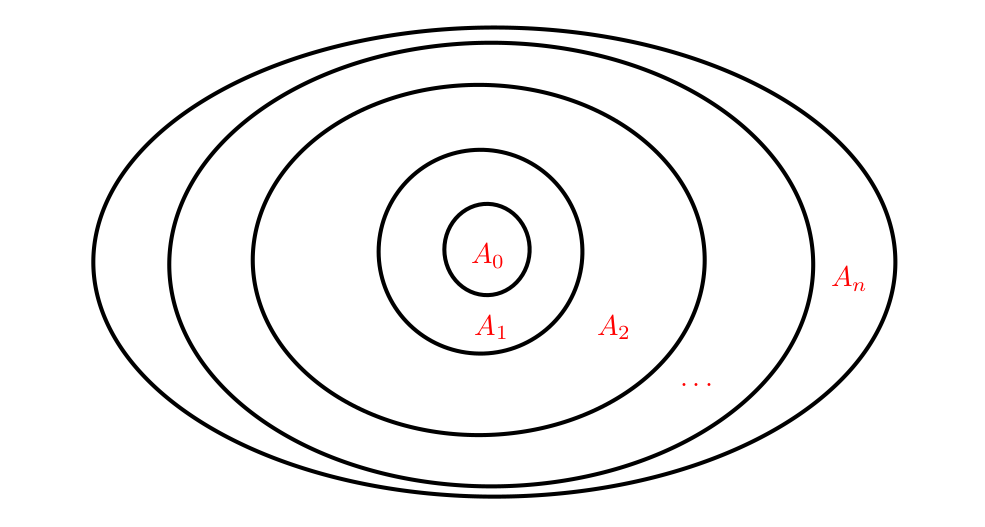
\includegraphics[scale=0.3]{figures/mesure-suite-ens.png}
    \caption{On construit ainsi les couronnes}
    \label{fig:mesure-suite-ens}
  \end{figure}


  Donc par le deuxième axiome, on a

  \begin{gather*}
    \mathbb{P}( \bigcup _{n=1} ^{\infty} A_n ) = \mathbb{P}( A_1 ) + \sum_{n=1}^{\infty} \mathbb{P}( A _{n+1} \setminus A_n ) \\
    = \mathbb{P}( A_1 ) + \lim_{k \to + \infty} \sum_{n=1}^{k} \mathbb{P}( A _{n+1} \setminus A_n ) \\
    =\mathbb{P}( A_1 ) + \lim_{k \to + \infty} \sum_{n=1}^{k} (\mathbb{P}( A _{n+1} ) - \mathbb{P}( A_n ) ) \text{ (somme téléscopique) }
  \end{gather*}

  Or on a

  \begin{gather*}
    \sum_{n=1}^{k} (\mathbb{P}( A _{n+1} ) - \mathbb{P}( A_n ) )  = \mathbb{P}( A _{k+1} ) - \mathbb{P}( A_1 ).
  \end{gather*}

  Donc

  \begin{gather*}
    \mathbb{P}\left( \bigcup _{n=1} ^{\infty} A_n \right) = \mathbb{P}( A_1 ) + \lim_{k \to \infty} [\mathbb{P}( A _{k+1} ) - \mathbb{P}( A_1 )]
  \end{gather*}

  et on obtient le résultat désiré.
\end{proof}

$(\Omega, \mathscr{A}, \mathbb{P} )$ espace mesuré ou de probabilité.

Dans le langage des probabilités, on appelle $\Omega$ l'univers et les éléments de $\mathscr{A} $ sont des événements.

\section{Mesure de Dirac}

Soit $\omega _{0} \in \Omega$ quelconque.

$\delta  _{w_0}(A), A \in \mathscr{A} $.

$\delta _{w_0}(A) =
 \begin{cases}
  1 \text{ si } w_0 \in A \\
  0 \text{ sinon}.
\end{cases}$

Montrer qu'il s'agit d'une probabilité.

\

 Soit $\Omega = \{ \omega_1, \omega_2, \dots, w_k, \dots \} $.

 On associe à $w_i$ un poids $p_i$ tel que

 \begin{equation}
   \sum_{i=1}^{\infty} p_i = 1.
 \end{equation}

 Si $A \subset \Omega$, on définit

 \begin{equation*}
   \mathbb{P}( A ) = \sum_{i,  \omega_i \in A}^{} p_i.
 \end{equation*}

 Si $card(\Omega) \less \infty$, $\Omega = \{ \omega_1, \omega_2, \dots, \omega _{N} \} $.

 On associe à $\omega _{j} = \frac{1}{N}$.

 Donc

 \begin{gather*}
   \mathbb{P}( A ) = \sum_{i, \omega_i \in A}^{} \frac{1}{N} = \frac{card(\omega_i \text{ dans } A)}{card(\text{total de } \omega_i )} = \frac{\text{ cas favorables } }{\text{ cas possibles } }.
 \end{gather*}

\section{Mesure de Lebesgue}

Elle est définie sur $\beta (\mathbb{R})$ et elle est la seule mesure qui se comporte comme ceci :

$\lambda ( (a,b] ) = b-a$.

On a aussi

\begin{equation}\label{lebesgue-zero}
  \lambda ((a,b)) = \lambda ([a,b]) = b-a.
\end{equation}

$(a,b] = (a,b) \cup \{ (b)\}$.

Il faut montrer que $\lambda (\{ b \} ) = 0$.

On a

\begin{gather*}
  \{ b \} = \bigcap _{n=1} ^{\infty} (b- \frac{1}{k}, b].
\end{gather*}

Donc

\begin{gather*}
  \lambda (\{ b \} ) = \lambda (\bigcap _{k=1} ^{\infty} (b - \frac{1}{k}, b]) \text{ intersection décroissante } \\
  = \lim_{k \to \infty} \lambda ((b- \frac{1}{k}, b]) \\
  = \lim_{k \to \infty} (b-b+ \frac{1}{k}) = \lim_{k \to \infty} \frac{1}{k} = 0.
\end{gather*}

\subsection{Mesure de Lebesgue-Stieltjes}

Soit $F$ une fonction croissante bornée et continue à droite (i. e. $F(x_0) = \lim_{x \to x_0} F(x)$) et supposons que

\begin{figure}[h!]
  \centering
  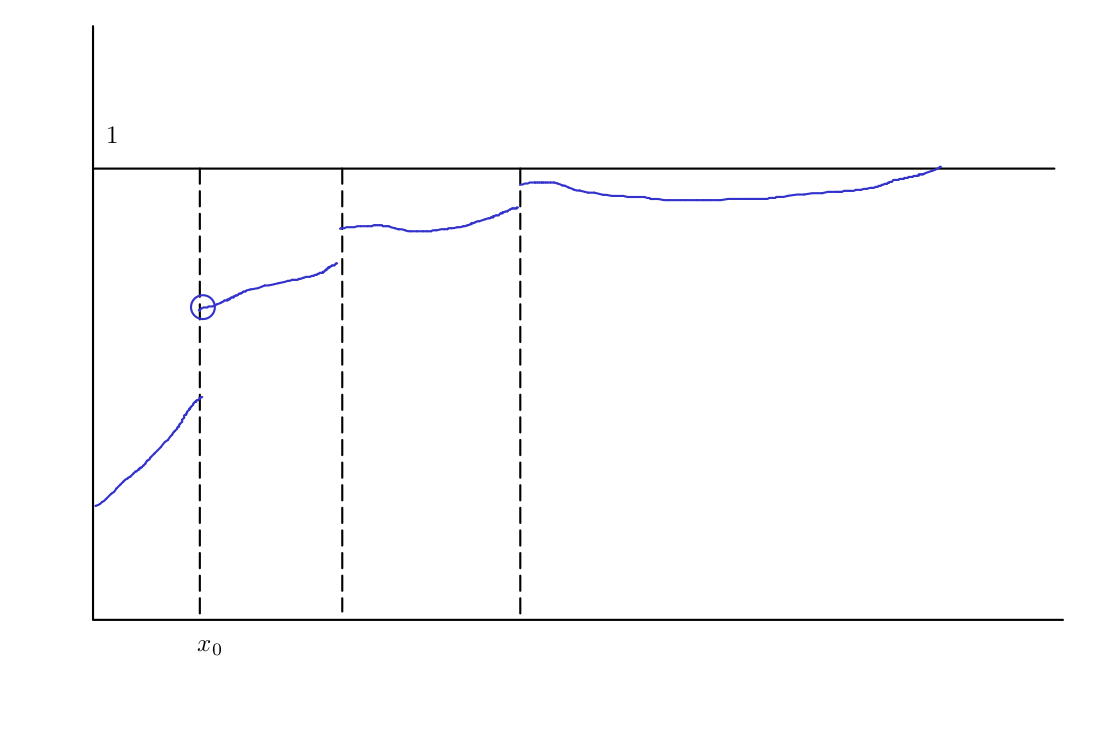
\includegraphics[scale=0.2]{figures/lebesgue-stieltjes}
  \caption{Mesure de Lebesgue-Stieltjes}
  \label{}
\end{figure}

On définit une fonction d'ensemble $\nu ((a,b]) = F(b) - F(a)$. $\nu$ devient une mesure de probabilité sur $\sigma((a,b]) = \beta $.

On a $\nu(\{ x_d \} ) \neq 0$.

\begin{proof}
  $\{ x_d \} = \bigcap_{k=1} ^{\infty} (x_d - \frac{1}{k}, x_d] $.

  Or
  \begin{gather*}
    \nu(\{ x_d \} ) = \lim_{k \to \infty} \nu((x_d - \frac{1}{k}, x_d]) = \lim_{k \to \infty} F(x_d) - F(x_d - \frac{1}{k}) \\
    = F(x_d) - \lim_{k \to \infty} F(x_d - \frac{1}{k})  = F(x_d) _{+} - F(x_d) _{-} \\
    = \text{ différence entre la limite gauche et la limite droite } \bg 0.
  \end{gather*}
\end{proof}

\section{Fonctions mesurables}

$(\Omega, \mathscr{A} ) \to (\mathbb{R}, \beta )$, $f : \Omega \to \mathbb{R}$.

\begin{definition}[Mesurable]
  On dit que $f$ est mesurable si pour tout borélien $B \in \beta $, $f ^{-1} (B) \in \mathscr{A} $.
\end{definition}

\begin{definition}[Equivalente]
  $f ^{-1} (\beta )$ est une sous $\sigma$-algèbre de $\mathscr{A} $.
\end{definition}

\begin{exo}
  Montrer que $f ^{-1} (\beta )$ est une $\sigma$-algèbre.
\end{exo}

\begin{proof}
  \begin{enumerate}
    \item $f ^{-1} (\mathbb{R}) = \Omega$.
    \item Si $A \in f ^{-1} (\beta )$, est-ce que $A ^{C}$ est aussi dans $f ^{-1} (\beta )$ ?

    Si $A \in f ^{-1} (\beta )$, alors $\exists B \in \beta $ tel que $A = f ^{-1} (B)$.

    $A ^{C} = (f ^{-1} (B)) ^{C} = f ^{-1} (B ^{C})$.

    \item Si $\{ A_n \} \in f ^{-1} (\beta ) $, est-ce que $\bigcup_{n=1} ^{\infty} A_n \in f ^{-1} (\beta ) $ ?
  \end{enumerate}
\end{proof}

\begin{prop}
  $f : \Omega \to \mathbb{R}$.

  Soit $\mathscr{C} $ une famille dans $\mathbb{R}$ telle que $\sigma(\mathscr{C} ) = \beta $.

  Si $ f ^{-1} (C ) , C \in \mathscr{C} $ est dans $\mathscr{A} $, alors $f$ est mesurable.
\end{prop}

\begin{exemple}
  $f : \Omega \text{ (topologie) }  \longrightarrow \mathbb{R} \text{ (topologie ouverts) } $ continue.

  $f$ est mesurable.

  Si $\mathcal{O}$ ouvert dans $\mathbb{R}$, $f ^{-1} (\mathcal{O})$ est ouvert dans $\Omega$.
\end{exemple}

\

$f : (\Omega, \mathscr{A} ) \longrightarrow (\mathbb{R}, \beta )$. Pour tout $\omega \in \Omega$, $f(\omega) = \text{ constante. } $

On a deux cas :

\begin{enumerate}
  \item $f ^{-1} ((a,b)) = \emptyset$ si la constante n'est pas dans $(a,b)$;
  \item $f ^{-1} ((a,b)) = \Omega$ si la constante est bien dans $(a,b)$.
\end{enumerate}

\begin{exemple}
  Soient $f, g : (\Omega, \mathscr{A} ) \to (\mathbb{R}, \beta )$ deux fonctions mesurables. Montrons que $f+g$ est mesurable.
\end{exemple}


\begin{proof}
  On considère la famille $\{ (a, \infty) \}$.

  Si on veut montrer que $f+g$ est mesurable, il suffit de montrer que $(f+g) ^{-1} ((a, \infty)) \in \mathscr{A} $.

  Donc il faut montrer que $\{ \omega, f(\omega) + g(\omega) \bg a \} \in \mathscr{A}  $, ie $\{ \omega, f(\omega) \bg a - g(\omega) \} $.

  Montrons d'abord que $a - g$ est mesurable.

  $\omega \in (a - g) ^{-1} ((b, \infty))$.

  \begin{gather*}
    a - g(\omega) \bg b \implies - g(\omega) \bg b-a \\
    \text{Or }\{ \omega, g(\omega) \less a-b \} \in \mathscr{A}, \\
    \text{c'est à dire } g ^{-1} ((- \infty, a-b)) \in \mathscr{A} .
  \end{gather*}

  Notons $h = a - g$.

  Si $f, h$ sont mesurables, est-ce que $\{ \omega, f(\omega) \bg h(w) \} $ ?

  On a $\{ \omega, f(\omega) \bg h(x) \} = \bigcup_{r \in \mathbb{Q}} \{ f \bg r \} \cap \{ h \less r \} $.

  Or $\{ \omega, f(\omega) \bg r \} = f ^{-1} (r, \infty)  \in \mathscr{A} $ et $\{ \omega, h (\omega) \less r \} = h ^{-1} ((-\infty, r)) \in \mathscr{A}  $.

  On a donc montré que $f+g$ est mesurable.
\end{proof}

\begin{prop}
  On a aussi :
  \begin{enumerate}
    \item Si $\lambda $ est un scalaire, $\lambda f$ est mesurable ;
    \item $f \cdot g$ est mesurable ;
    \item Si $g \neq 0$, $\frac{f}{g}$ est mesurable ;
    \item Si on a une suite $\{ f_n \} _{n \in \mathbb{N}} $ de fonctions mesurables, on a $\sup f_n, \inf f_n, \lim \sup f_n, \lim \inf f_n$ sont mesurables.
  \end{enumerate}
\end{prop}

Soient $\Omega \in \mathbb{R}$ borné et $f : (\Omega, \beta ) \longrightarrow (\mathbb{R}, \beta )$.

Soit $\mathcal{P}$ une partition de $\Omega$, ie un ensemble $\mathcal{P} = \{ P_i \} _{i=1} ^{\infty} $ tel que $$\bigcup_{i=1} ^{\infty} P_i = \Omega \text{ et } P_i \cap P_j \neq 0 \text{ si } i \neq j. $$

Considérons par exemple la partition $\mathcal{P} = \{ P_1, P_2, P_3, P_4 \} $.

Comme $\mathcal{P}$ est une famille dans $\Omega$, construisons $\sigma(\mathcal{P})$, ie la $\sigma$-algèbre engendrée par $\mathcal{P}$.  Dans notre cas, $\sigma(P_1, P_2, P_3, P_4)$.

Cette $\sigma$-algèbre est composée par la réunion d'éléments de $\mathcal{P} \cup \{ \emptyset \}$.

\begin{gather*}
  \sigma(\mathcal{P}) = \{ \emptyset, \Omega, P_1, P_2, P_3, P_4, P_1 ^{C} = P_2 \cup P_3 \cup P_4, \dots  \}.
\end{gather*}

Si on a $B = \bigcup_{i=1} ^{m} P_i $, alors $B ^{C} = \bigcap_{i=1} ^{m} P_i ^{C} = \bigcap_{i=1}^{m} \left(\bigcup_{i=1}^{m} P_i\right)   $.

\begin{prop}
  On sait exactement comment sont faites les fonctions mesurables dans ce cas. Il s'agit de fonctions constantes par morceaux.
\end{prop}

\begin{proof}
  Soit $ \{ p \} \in \mathbb{R}$, donc $f ^{-1} (\{ p \} ) \in \sigma(\mathcal{P})$.

  Supposons par exemple que $f ^{-1} (\{ p \} ) = P_2 \cap P_3$. Si $x \in f ^{-1} (\{ p \} )$, alors $ f(x) = p$, mais $x \in P_2 \cup P_3$, donc sur $P_2 \cup  P_3$ on aura en fait une valeur constante.

   %donc si $x \in f ^{-1} (\{ p \} ), f(x)=p, x \in P_2 \cup P_3$.
\end{proof}

\

\begin{definition}[Variable aléatoire]
  Soit $X : (\Omega, \mathscr{A}, \mathbb{P} ) \longrightarrow (\mathbb{R}, \beta )$.

  Si $X$ est une fonction mesurable, on dit que $X$ est une \textbf{variable aléatoire}.
\end{definition}

\begin{remark}[Notations]
  On notera

  $$\mathbb{P}( X \in B ) = \mathbb{P}( \omega, X(\omega) \in B ). $$

\end{remark}



\section{Loi de la variable aléatoire}

\begin{definition}[Loi de variable aléatoire]\label{loi_va}
  Il s'agit d'une mesure de probabilité définie sur $\mathbb{R}$. On va la noter avec le symbole $P_X$.

  Si $B \in \beta $, $$P_X(B) = \mathbb{P}( X ^{-1} (B) ),$$ avec $$X ^{-1} (B) = \{ \omega \mid X(\omega) \in B \}.$$
\end{definition}



\begin{definition}[Rappel : mesure (cf cours d'intégration de L3)]

  \

  Soit $(E, \tau)$ un ensemble mesurable. Alors une application $\mu : \tau \to \overline{\mathbb{R} ^{+}} $ est une mesure sur $E$ si :
 \begin{enumerate}
   \item $\mu(\emptyset) = 0$;
   \item Pour toute suite $(A_n)$ de $\tau$ disjointe, ie $A_n \cap A_m = \emptyset$ si $m \neq n$, alors $$\mu \left(\bigcup_{n \in \mathbb{N}} A_n \right) = \sum_{n \in \mathbb{N}} \mu(A_n) \ (\sigma \text{-additivité.})$$
 \end{enumerate}
\end{definition}

\begin{figure}[h!]
  \centering
  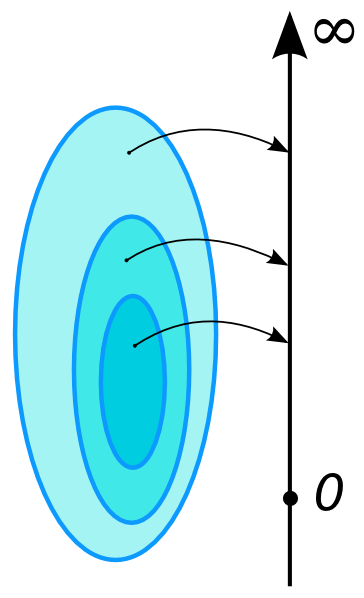
\includegraphics[scale=0.3]{figures/Measure_illustration.png}
  \caption{De façon informelle, une mesure a la propriété d'être monotone : si l'ensemble $ E$ est un sous-ensemble de $ F$, la mesure de $ E$ est inférieure ou égale à celle de $ F$. De plus, on impose à la mesure de l'ensemble vide la valeur 0 (Wikipédia).}
  \label{}
\end{figure}

\begin{exo}
  Montrer que $P_X$ est une mesure.
\end{exo}

\begin{proof}
  \begin{enumerate}
    \item $P_X(\mathbb{R}) = \mathbb{P}( X ^{-1} (\mathbb{R}) ) = \mathbb{P}( \Omega ) = 1$ ;
    \item Si $\{ B_n \} $ est une suite deux à deux disjointe,

    \begin{gather*}
      P_X \left( \bigcup _{n=1} ^{\infty} B_n \right) = \sum_{n=1}^{\infty} P_X(B_n),
    \end{gather*}

    car

    \begin{gather*}
      P_X \left(\bigcup _{n=1} ^{\infty} B_n \right) = \mathbb{P}\left( X ^{-1} \left(\bigcup _{n=1} ^{\infty} B_n \right) \right) \\
      = \mathbb{P} \left( \bigcup _{n=1} ^{\infty} X ^{-1} (B_n) \right) \text{ (propriété de l'image réciproque) }  \\
      = \sum_{n=1}^{\infty} \mathbb{P}( X ^{-1} (B_n) ) \ (\mathbb{P} \text{ est une probabilité} ) \\
      = \sum_{n=1}^{\infty} P_X (B_n).
    \end{gather*}
  \end{enumerate}
\end{proof}

\marginpar{15-09-2023}

\section{Intégrale}

\begin{definition}[Fonctions étagées/simples]
  Soit $X$ espace mesuré, $x \in X$. Une fonction $h$ est appelée fonction étagée si $h$ s'écrit de la manière suivante

  $$ h(x) = \sum_{k=1}^{M} c_k \mathds{1} _{A_k}(x), $$

  avec $A_k$ ensemble mesurables (un élément de la $\sigma$-algèbre) tel que $A_k \cap A_j$ si $k \neq j$ et $c_k \geq 0$.


\end{definition}

\begin{thm}
  Soit $f : (X, \mathscr{A}, \mu )$ (espace mesuré) $\longrightarrow (\mathbb{R} ^{+}, \beta )$ mesurable.

  Alors il existe une suite croissante $(\forall x, h_n(x) \leq h _{n+1}(x))$ de fonctions étagées  $\{ h_k \} _{n \in \mathbb{N}}$ telle que

  \begin{gather*}
    f(x) = \lim_{n \to \infty} h_n(x).
  \end{gather*}
\end{thm}

\begin{definition}[Intégrale de Lebesgue]

  \

  \begin{enumerate}
    \item \emph{Première étape.} On considère une fonction simples

    $$ h(x) = \sum_{k=1}^{M} c_k \mathds{1} _{A_k}(x), $$

    alors $$ \int_{X}^{} h d \mu = \int_{X}^{}h(x) d \mu(x) = \sum_{k=1}^{M} c_k \mu(A_k).$$

    \item \emph{Deuxième étape.} Si $f$ est mesurable non négative,

    \begin{enumerate}
      \item $$ \int_{X}^{} f d \mu = \sup \left( \int_{X}^{} h d \mu, h \text{ simple, } h \leq f \right). $$
      \item Si $f = \lim_{k \to \infty} h_k, h_k $ simples non négatives,

      $$ \int_{X}^{} f d \mu = \lim_{k \to \infty} \int_{}^{} h_k d \mu.$$
    \end{enumerate}

    \item Si $f$ mesurable de signe quelconque, on écrit $f(x) = f _{+}(x) - f _{-}(x)$, où $f _{+} = \max (f,0)$ et $f _{-} = \max (-f, 0)$.

    (à suivre...)

  \end{enumerate}
\end{definition}

\begin{definition}[De classe $\mathscr{L} ^{1}$]
  On dira que $f$ est de classe $\mathscr{L} ^{1} $ si

  $$ \int_{X}^{} \lvert f \rvert d \mu \less +\infty. $$

  Dans ce cas, $\lvert f \rvert = f _{+} + f _{-}$.
\end{definition}


\begin{exemple}
  On considère la mesure de Dirac

  %\begin{figure}[h!]
  %  \centering
  %  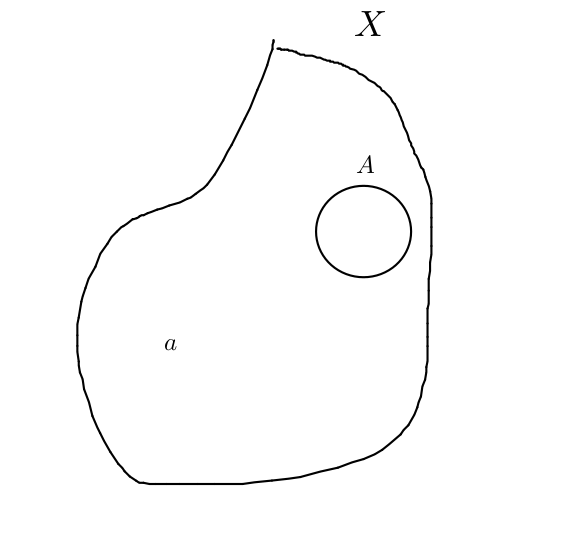
\includegraphics[scale=0.3]{figures/L1.png}
  %  \caption{}
  %  \label{}
  %\end{figure}

  $$ \delta _a (A) = \begin{cases}
    1 \text{ si } a \in A \\
    0 \text{ sinon. }
  \end{cases}$$

  Alors \begin{equation}\label{int_dirac}
     \int_{X} f(x) d \delta _a(x) = f(a) .
  \end{equation}
\end{exemple}



\begin{proof}
  Soit $f = \sum_{k=1}^{M} c_k \mathds{1} _{A_k}$ une fonction simple.

  \begin{gather*}
    \int_{}^{} \sum_{k=1}^{M} c_k \mathds{1} _{A_k}(x) d \delta _a(x) = \sum_{k=1}^{M} c_k \delta _a(A_k) = c _{\overline{k} } \\
     \text{ avec } \overline{k} \text{ le seul } k \text{ tel que } a \in A _{k } \text{ car les } A_k \text{ sont deux à deux disjoints. }
  \end{gather*}

  Or $c _{\overline{k} } = f(a)$.

  \begin{figure}[h!]
    \centering
    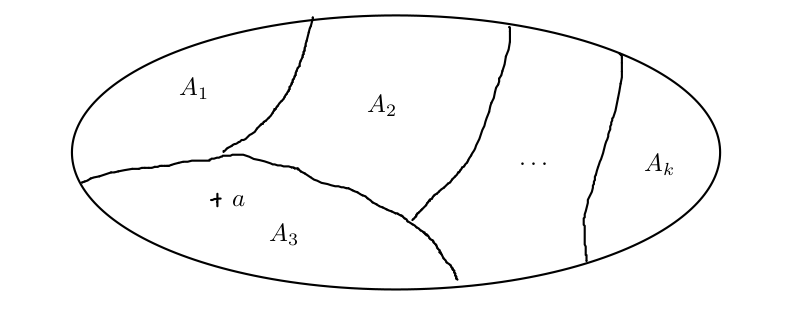
\includegraphics[scale=0.3]{figures/fct_etagees_ak.png}
    \caption{$a$ ne peut être que dans un seul des $A_k$.}
    \label{}
  \end{figure}

  \

  On suppose maintenant que $f(x) = \lim_{k \to \infty} h_k(x) $.

  Alors

  \begin{gather*}
    \int_{X}^{} f(x)d \delta _a(x) = \int_{X}^{} \lim_{k \to \infty}h_k(x) d \delta _a(x) \stackrel{\text{Beppo-Levi}}{=} \lim_{k \to \infty} \int_{X}^{} h_k d \delta _a(x) = \lim_{k \to \infty} h_k(a)= f(a).
  \end{gather*}
\end{proof}

\begin{thm}[Beppo-Levi]
  Si $\{ h_k \} $ est une suite monotone non négative, alors

  $$ \lim \int f_k = \int_{}^{} \lim_{ } f_k.$$
\end{thm}

\begin{remark}
  Si $\mu = \sum_{k=1}^{M} p_k \delta _{a_k} $, avec $\sum_{k=1}^{M} p_k = 1 $, alors

  $$ \int_{X}^{} f d \left(\sum_{k=1}^{M} p_k \delta _{a_k}  \right) = \sum_{k=1}^{M} p_k f(a_k).$$
\end{remark}

\begin{proof}
  Même démonstration que pour \ref{int_dirac}.
\end{proof}

\subsection{Conséquences en probabilités}


Soit $X : (\Omega, \mathscr{A}, \mathbb{P} ) \longrightarrow (\mathbb{R}, \beta)$.

$X$ est une variable aléatoire. Associée à $X$, il y a une mesure de Borel sur la droite qu'on appelle la loi notée $P_X$ (cf \ref{loi_va}).

\begin{definition}[Espérance de $X$]
  L'espérance de $X$ se calcule comme suit :

  \begin{equation}
    \mathbb{E}[ X ] = \int_{\Omega}^{} X(\omega) d \mathbb{P}( \omega ).
  \end{equation}
\end{definition}

\begin{thm}[De transfert]
  On a

  \begin{equation}
    \int_{\Omega}^{} f(X(\omega)) d \mathbb{P}( \omega ) = \int_{\mathbb{R}}^{} f(x) d P_X(x), \text{ avec } x \in \mathbb{R}.
  \end{equation}
\end{thm}

\begin{proof}
  Soit $f : \mathbb{R} \to \mathbb{R}$ fonction simple telle que $f(x) = \sum_{k=1}^{M} c_k \mathds{1} _{A_k}(x) $.

    \begin{figure}[h!]
      \centering
      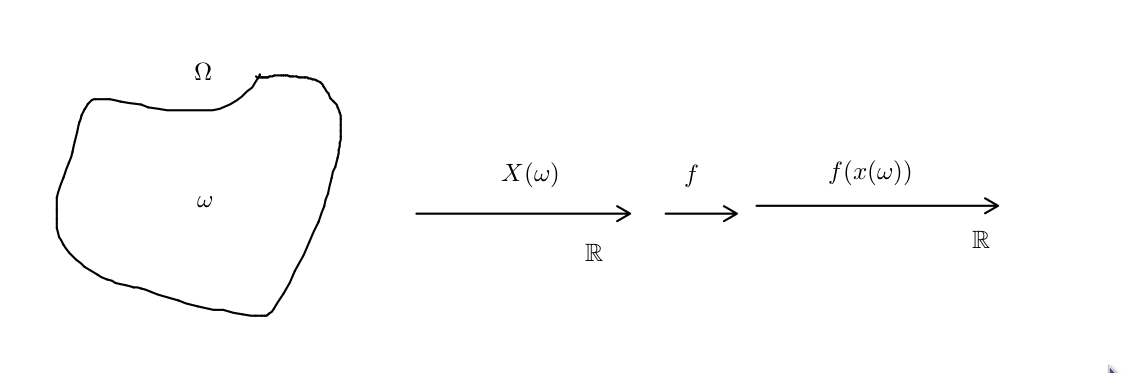
\includegraphics[scale=0.3]{figures/transfert.png}
      \caption{Illustration théorème de transfert}
      \label{}
    \end{figure}

  \begin{gather}\label{transfert-1}
    \int_{\Omega}^{} \sum_{k=1}^{M} c_k \mathds{1} _{A_k}(X (\omega)) d \mathbb{P}( \omega )  = \sum_{k=1}^{M} c_k \int_{\Omega}^{} \mathds{1} _{A_k}(X(\omega)) d \mathbb{P}( \omega ).
  \end{gather}

  Or

  \begin{gather*}
    \int_{\Omega}^{} \mathds{1} _{A_k}(X (\omega)) d \mathbb{P}( \omega ) = \int_{\Omega}^{} \mathds{1} _{X ^{-1} (A_k)}(\omega) d \mathbb{P}( \omega ) = \mathbb{P}( X ^{-1} (A_k) ) = P_X (A_k)
  \end{gather*}

  Donc \ref{transfert-1} devient :

  \begin{gather*}
    \sum_{k=1}^{M} c_k P_X(A_k) = \int_{\mathbb{R}}^{} f(x) d P_X(x).
  \end{gather*}

  \

  On considère que $f$ est quelconque avec $f = \lim_{k \to \infty} h_k$, avec $\{ h_k \} $ suite de fonctions simples.

  \begin{gather*}
    \int_{}^{} f(X(\omega)) d \mathbb{P}( \omega ) = \int_{}^{} \lim_{k \to \infty}   h_k(X(\omega)) d \mathbb{P}( \omega ) = \lim_{k \to \infty} \int_{}^{} h_k (X(\omega)) d \mathbb{P}( \omega ) \\
    =\lim_{k \to \infty} \int_{\mathbb{R}}^{} h_k(x) d P_X(x) =  \int_{\mathbb{R}}^{} \lim_{k \to \infty} h_k(x) d P_X(x) = \int_{\mathbb{R}}^{} f d P_X
  \end{gather*}

\end{proof}

\section{Fonctions de répartition}

\begin{definition}[Fonction de répartition]
  Soit $X : \Omega \longrightarrow \mathbb{R}$ une variable aléatoire. On définit

  \begin{gather}
    F(t) = \mathbb{P}( X \leq t ), t \in \mathbb{R} \\
    = \mathbb{P}( \omega, X(\omega) \leq t ) = \mathbb{P}( X ^{-1} ((-\infty, t]) ) = P_X((-\infty, t]).
  \end{gather}
\end{definition}



\begin{figure}[h!]
  \centering
  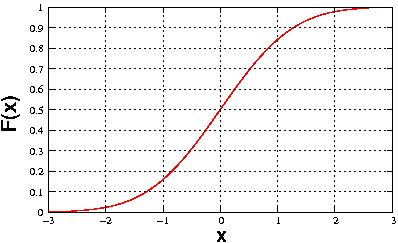
\includegraphics[scale=0.5]{figures/F_repartition.png}
  \caption{Fonction de répartition}
  \label{}
\end{figure}

\begin{prop}[Propriétés de $F$]

  \

  \begin{enumerate}
    \item $F$ est non négative et bornée entre 0 et 1.
    \item $F$ est croissante et continue à droite.
    \item $$ \begin{cases}
      \lim_{t \to +\infty} F(t) = 1 \\
      \lim_{t \to -\infty} F(t) = 0.
    \end{cases}$$
    \item $F$ est discontinue dans au plus un nombre dénombrable de points.
  \end{enumerate}
\end{prop}

\begin{proof}
  \begin{enumerate}
    \item \emph{Continuité à droite.} Si $a$ est un point de discontinuité,

    \begin{equation*}
      F(a) = \lim_{t \to a ^{+}} F(t).
    \end{equation*}

    \begin{equation*}
      F(a) = P_X((-\infty, a]) = P_X \left( \bigcap _{k=1} ^{\infty} \left(-\infty, \frac{1}{k}\right) \right) = \lim_{k \to \infty} P_X\left(\left(-\infty, a+ \frac{1}{k}\right)\right) = \lim_{k \to \infty} F\left(a+ \frac{1}{k}\right) = \lim_{t \to a ^{+}} F(t),
    \end{equation*}

    car on écrit
  \begin{gather*}
    (-\infty, a] = \bigcap _{k=1} ^{\infty} \left(-\infty, a + \frac{1}{k}\right).
  \end{gather*}
  \end{enumerate}
\end{proof}

Soit $\pi(a)$ le saut dans un point de discontinuité de la fonction de répartition. On définit

$$A_n = \{ t \in \mathbb{R}, \pi(t) \geq  \frac{1}{n} \}. $$

Comme $F$ est bornée entre 0 et 1, il peut y avoir au plus $n$ éléments dans $A_n$.

Les points de discontinuité sont données par des points $$ t \in \bigcup_{n \geq 1} A_n \text{ (ensemble dénombrable). } $$

Comme $F$ est continue et croissante à droite, elle définit une mesure de Lebesgue-Stieltjes

$$ \nu((a,b]) = F(b) - F(a).$$

\begin{proof}
  Montrons que $\nu = P_X$.
  \begin{gather*}
    P_X((a,b]) = P_X((-\infty, b]) - P_X((-\infty, a]) = F(b)-F(a).
  \end{gather*}
\end{proof}


\marginpar{18-09-2023}

$\mathbf{\nu}$ \textbf{ne peut avoir que deux formes particulières.}



\begin{enumerate}
  \item $\nu$ est une somme de masses de Dirac. Si $A$ est un borélien de $\mathbb{R}$, alors

  \[
  \nu(A) = \sum_{k=1}^{\infty} p_k \delta _{X_k}(A),
  \]

  avec

  \[
  \sum_{k=1}^{\infty} p_k = 1.
  \]


  Alors

  \[
  p_k = \mathbb{P}(X = \{ x_k \} ) = \mathbb{P}(\omega, X(\omega) = x_k).
  \]


  \begin{definition}[Variable aléatoire discrète]
    On appelle \textbf{discrète} toute variable aléatoire $X$ dont la loi a la forme :

    \begin{equation*}
      P_X = \sum_{k=1}^{\infty} p_k \delta _{X_k}(A).
    \end{equation*}

    En particulier, nous écrirons toute variable aléatoire

    \[
    X(\omega) = \sum_{k=1}^{\infty} x_k \mathds{1} _{A_k}(\omega) \text{ et on aura } P_X(A) = \sum_{k=1}^{\infty} p_k \delta _{x_k}(A), \text{ avec }  p_k = \mathbb{P}( A_k ).
    \]

  \end{definition}

  \begin{figure}[h!]
    \centering
    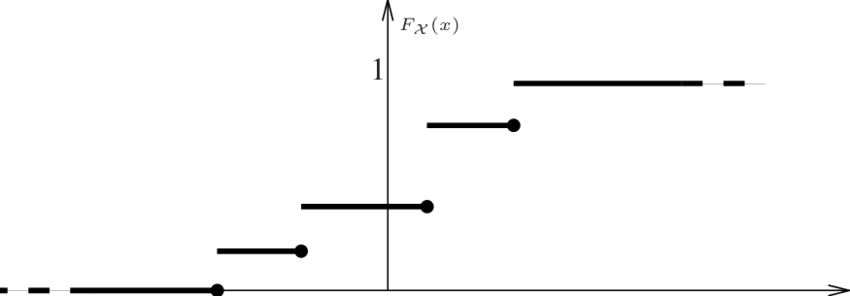
\includegraphics[scale=0.3]{figures/fct-rep-disc.png}
    \caption{Exemple de fonction de répartition d'une variable aléatoire discrète.}
    \label{}
  \end{figure}

  \begin{remark}[Notations]
    Mesure de Lebesgue :   $\begin{cases}
      \text{Leb} \\
      dx
    \end{cases}$
  \end{remark}

  \item Soit $\nu$ une mesure de probabilité de Borel sur $\mathbb{R}$. On dira que $\nu$ est \textbf{absolument continue} s'il existe une fonction non-négative $f \in L ^{1}(\text{Leb}) \ (\int_{\mathbb{R}}^{} f dx \less \infty )$ telle que, pour tout borelien $B$,

  \begin{equation*}
    \nu(B) = \int_{B}^{} f(x) dx.
  \end{equation*}

  \emph{On la dénote aussi $\nu \ll \text{Leb}$.}

  En particulier si $g$ est bornée ($L ^{\infty}(\text{Leb})$), alors

  \begin{equation*}
    \int_{\mathbb{R}}^{} g d \nu = \int_{\mathbb{R}}^{} gf dx.
  \end{equation*}

  $f$ est la densité de $f$ par rapport à Lebesgue (dérivée de Radon-Nykodym).

\end{enumerate}

Dans notre cas, $\nu((a,b]) = F(b)-F(a)$.

Si $F$ est la fonction de répartition de $X$, on a

\begin{gather*}
  P_X((a,b]) = F(b)-F(a) \stackrel{\text{Si la loi est AC}}{=} \int_{(a,b]}^{} f(x)dx \\
   = \int_{[a,b]}^{} f(x) dx = \underbrace{\int_{a}^{b} f(x) dx }_{\text{Intégrale de Riemann}}
\end{gather*}

\begin{definition}[Variable aléatoire à densité]
  On dira qu'une variable aléatoire $X$ est \textbf{à densité} si sa loi est absolument continue et on appelle $f_X$ la densité de probabilité de $X$.
\end{definition}

Si $\nu = c_1 \delta _{X_1} + c_2 \text{Leb}$, on écrit $\nu(A) = c_1 \delta _{X_1}(A) + c_2 \text{Leb} (A)$.

Il n'y a pas de saut dans la fonction de répartition d'une variable aléatoire absolument continue, car si $F(b) - F(a) = \int_{a}^{b} f(t) dt $, on a $$\text{saut}(x_0) = F(x_0) - F(x_0 ^{-}) = 0.$$

C'est lié au fait que pour $\lambda$ mesure de Lebesgue, on a $\lambda (\{ b \} ) = 0$ (cf \ref{lebesgue-zero}).

\begin{thm}
  Toute fonction de répartition $F$ s'écrira (pour nous) de la forme

  \begin{equation*}
    F(t) = c_1 F _{\text{d} }(t) + c_2 F _{\text{ac}}(t),
  \end{equation*}

  où $F _{\text{d}}$ est la fonction de répartition d'une variable aléatoire discrète et $F _{\text{ac}}$ est la fonction de répartition d'une variable aléatoire absolument continue et $c_1+c_2 = 1$.
\end{thm}

Dans ce cas, $P_X = c_1 (\text{masses de Dirac}) + c_2(\text{mesure absolument continue})$.

\

Soit $X$ une variable à densité $f_X$. Soit $g :  \mathbb{R} \to \mathbb{R}$. On considère la même variable aléatoire $g \circ X$. Quelle est sa loi ?


\begin{exemple}
  Soit une variable aléatoire $X$ avec la loi exponentielle. $X : \Omega \longrightarrow \mathbb{R}$,

  \begin{gather*}
    f_X(x) = e^{-x} \mathds{1} _{[0, \infty)}(x).
  \end{gather*}

  Trouver la loi de $X ^2 = g \circ X$, avec $g : x \to x ^2$.
\end{exemple}

Soit $h$ une fonction bornée positive quelconque (fonction test).

\begin{gather}
  \int _{\Omega} h(g(X)) d \mathbb{P} = \int _{\Omega} (h \circ g) (X) d \mathbb{P} \stackrel{\text{transfert}}{=} \int_{\mathbb{R}} (h \circ g)(x) d P_X(x) \\
  = \int_{\mathbb{R}}^{} (h \circ g)(x) f_X(x) dx = \int_{A}^{} h(g(x)) f_X(x) dx. \label{chgt-var}
\end{gather}

On fait un changement de variable en posant $y=g(x), d y = g'(x) dx$.

Dans ce cas, \ref{chgt-var} devient

\begin{gather*}
\int h(y) f_X (g ^{-1} (y)) dy.
\end{gather*}

Or

\begin{gather*}
  \int h(y) c(y) dy = \int_{g(A)}^{} h(y)  f_X(g ^{-1} (y)) \frac{1}{g' (g ^{-1} (y))}dy,
\end{gather*}

avec $c$ la densité associée à $y = g(x)$ et $(g ^{-1} )' = \displaystyle\frac{1}{g'(g ^{-1})}$.


Comme $h$ est quelconque,

\begin{gather*}
  c(y) = f_X(g ^{-1}(y) ) \frac{1}{g' (g ^{-1} (y))} \mathds{1} _{g(A)} (y).
\end{gather*}

Dans notre exemple, $X$ a la densité $f_X(x) = e^{-x} \mathds{1} _{[0, \infty)}(x) $ et $g(x) = x ^2$, $A = [0, \infty)$.

On a

\[
\begin{matrix}
  y = x ^2 \\
  x= \sqrt{ y }.
\end{matrix}
\]


On obtient

\begin{gather*}
  \overbrace{c(y)}^{\text{densité} X ^2 } = e^{- \sqrt{ y } } \mathds{1} _{[0, \infty)}(y) \frac{1}{2 \sqrt{ y } } \mathds{1} _{g([0, \infty))}(y) \\
  = \frac{e^{-\sqrt{ y } } }{2 \sqrt{ y } } \mathds{1} _{[0, \infty)} (y),
\end{gather*}

car $g([0, \infty)) = [0, \infty)$.

\begin{exemple}
  $X$ suit la loi uniforme entre $[-1, 1]$.

  $f_X = \frac{1}{2}\mathds{1}_{[-1, 1]} $, car $\displaystyle \frac{1}{2} \int_{-1}^{1}dt = 1 $.  Calculer $X ^2$.
\end{exemple}

\begin{gather*}
  \int_{}^{} h(g(X)) d \mathbb{P} = \int_{}^{} (h \circ g) (X) d \mathbb{P} = \int_{-1}^{1} (h \circ g)(x) f_X(x) dx \\
  = \int_{-1}^{0} (h \circ g)(x) f_X(x) dx + \int_{0}^{1} (h \circ g)(x) f_X(x) dx \\
  = \int_{0}^{1}  h(y) f_X(- \sqrt{ y } ) \frac{1}{2 \sqrt{ y } } dy + \int_{0}^{1} h(y) f _{X} (\sqrt{ y } ) \frac{1}{2 \sqrt{ y } } dy \\
  = \int_{0}^{1} h(y) \frac{1}{2 \sqrt{ y } } [f_X(-\sqrt{ y } ) + f_X(\sqrt{ y } )] dy.
\end{gather*}

On a

\begin{equation*}
  \int h (g(X)) d \mathbb{P} = \int h(y) c_Y(y) dy,
\end{equation*}

avec

\begin{equation*}
  c_Y(y) = \frac{1}{2 \sqrt{ y } } [f_X(- \sqrt{ y } )+ f_X(\sqrt{ y } )] \mathds{1}_{[0, 1]}(y).
\end{equation*}

\

Soit $(\Omega, \mathscr{A}, \mathbb{P} )$ un espace probabilisé. Soit $B \in \mathscr{A}, \mathbb{P}(B) \bg 0 $.

On peut définir $\mathbb{P}(A \mid B)$, la probabilité conditionnelle de $A$ sachant $B$, définie comme suit :

\begin{equation*}
  \mathbb{P}(A \mid B) = \frac{\mathbb{P}(A \cap B)}{ \mathbb{P}(B)}.
\end{equation*}

\begin{exo}
  Si l'on fixe $B$, montrer que $\mathbb{P}(\cdot \mid B) \to [0, 1]$ est une probabilité.
\end{exo}

On dira que deux événements $A$ et $B$ sont \textbf{indépendants} si $\mathbb{P}(A \cap B) = \mathbb{P}(A) \iff \mathbb{P}(A \cap B) = \mathbb{P}(A) \mathbb{P}(B)$, avec $\mathbb{P}(B) \bg 0$.

\section{Système complet d'événements}


\begin{definition}
  Soit
  \[
  \Omega = \bigcup_{i=1} ^{\infty} A_i,
  \]

  avec $A_i \cap A_j = \emptyset$ si $i \neq j$ et $\forall i \geq  1, \mathbb{P}(A_i) \bg 0$.



  On appelle $ \displaystyle \{ A_i \} _{i=1} ^{\infty}$ un \textbf{système complet d'événements} (SCE).
\end{definition}

\begin{thm}[Formule des probabilités totales]
  Si $B \in \mathscr{A} $ quelconque, alors

  \begin{gather*}
    \mathbb{P}(B) = \sum_{i=1}^{\infty} \mathbb{P}(B \cap A_i) = \sum_{i=1}^{\infty} \mathbb{P}(B \mid A_i) \mathbb{P}(A_i).
  \end{gather*}
\end{thm}

\marginpar{22-09-2023}

\chapter{Vecteurs aléatoires}

On considère maintenant des variables aléatoires $X : (\Omega, \mathscr{A}, \mathbb{P} ) \longrightarrow \mathbb{R}^n$ (\bsc{Borel} engendrée par les ouverts).

On étudiera surtout les cas où $n=2$. On dénote un vecteur aléatoire $X \equiv (X_1, X_2)$ (parfois $(X, Y)$). Parfois on écrit, pour $i = 1, \dots, n$,

\[
X_i = \pi_i \circ X, \text{ où } \pi_i :  \mathbb{R}^n \to \mathbb{R}, \pi_i(x_1, \dots, x_n) = x_i.
\]

$\pi_i$ est une \textbf{projection}.

\begin{definition}[Loi d'un vecteur aléatoire]
  Soit $B$ un borélien de $\mathbb{R}^n$. Alors la loi de $X$ (loi conjointe) est définie ainsi :

  \[
  P_X (B) = \mathbb{P}(\omega \in \Omega, X(w) = (X_1(\omega), \dots, X_n(\omega)) \in B) = \mathbb{P}(X ^{-1} (B)).
  \]
\end{definition}

\emph{Est-il possible de calculer la loi de $X_1$?}

Si on connaît la loi du couple de variables aléatoires, il est possible de calculer les lois des deux variables. Par contre, on ne peut pas avoir la loi du couple en connaissant la loi des deux variables aléatoires.

\begin{definition}[Loi marginale]
  Si $D$ est un borélien de $\mathbb{R}$, la loi de $X$ est

  \begin{gather*}
    \underbrace{P _{X_1}(D)}_{\text{loi marginale}} = \mathbb{P}(X_1 \in D) = \mathbb{P}(\pi_1 \circ X \in D) = \mathbb{P}(X \in \pi_1 ^{-1} (D)) = P_X(\underbrace{\pi_1 ^{-1} (D)}_{\text{borélien}}).
  \end{gather*}
\end{definition}

\begin{remark}
  $\pi_i ^{-1} (D)$ est borélien, car $\pi_i$ est continue.
\end{remark}


\section{Fonction de répartition}

Dans le cas où $n=2$, $X = (X_1, X_2)$,

\begin{gather*}
  F_X(t_1, t_2) = \mathbb{P}(X_1 \leq t_1, X_2 \leq t_2) = P_X((-\infty, t_1] \times (-\infty, t_2]).
\end{gather*}


\begin{definition}
  On dira que le vecteur aléatoire $X$ est \textbf{absolument continu} s'il existe une fonction $f$ mesurable et \textbf{non-négative} définie comme $f : \mathbb{R}^2 \to \mathbb{R}$ telle que, pour tout borélien $B$ de $\mathbb{R}^2$, on a

  \[
  P _{X}(B) = P _{(X_1, X_2)}(B) = \iint_{B} \underbrace{f(x_1, x_2)}_{\text{densité du couple}} dx_1 dx_2
  \]

  et si $B = (-\infty, t_1] \times (-\infty, t_2]$, alors

  \begin{gather*}
    F_X(t_1, t_2) = \int_{-\infty}^{t_1} \int_{-\infty}^{t_2} f(x_1, x_2) dx_1dx_2 = \iint_{\mathbb{R}^2} f(x_1, x_2) \mathds{1}_{(-\infty, t_1]}(x_1) \mathds{1}_{(-\infty, t_2]}(x_2) dx_1 dx_2.
  \end{gather*}
\end{definition}

\begin{prop}

  \

  \begin{gather*}
    F _{X_1} (t_1) = \lim_{t_2 \to \infty} F _{(X_1, X_2)} (t_1, t_2)  \text{ et } F _{X_2} = \lim_{t_1 \to \infty} F _{(X_1, X_2)} (t_1, t_2).
  \end{gather*}
\end{prop}

\begin{proof}
  \begin{gather*}
    F _{X_1}(t_1) = \mathbb{P}(X_1 \leq t_1) = \mathbb{P}(X_1 \leq t_1, \underbrace{X_2 \in \mathbb{R}}_{\text{toujours vrai}}),
  \end{gather*}

  car

  \begin{gather*}
    \{  X_1 \leq t_1 \} = \{ \omega, X_1(\omega) \leq t_1 \} = \{ \omega, X_1(\omega) \leq t_1 \} \cap \Omega = \{ \omega, X_1 (\omega)\leq t_1 \} \cap \underbrace{X_2 ^{-1} (\mathbb{R})}_{X_2 \in \mathbb{R}}).
  \end{gather*}

  Donc

  \begin{gather*}
    F _{X_1}(t) = \mathbb{P}(X_1 \leq t_1, X_2 \in \mathbb{R}) = P _{X_1, X_2} ((- \infty, t_1] \times \mathbb{R}) = \lim_{k \to \infty} P _{X_1, X_2} ((-\infty, t_1] \times (-\infty, k]),
  \end{gather*}

  car
  \[
  \left((-\infty, t_1] \times \bigcup _{k=1} ^{\infty} (-\infty, k)\right) = (-\infty, t_1] \times \mathbb{R}.
  \]

  Ainsi

  \begin{gather*}
    \lim_{k \to \infty} P _{X_1, X_2} ((-\infty, t_1] \times (-\infty, k]) = \lim_{k \to \infty} F _{(X_1, X_2)} (t_1, k), k \in \mathbb{R}.
  \end{gather*}
\end{proof}

\begin{thm}[De transfert pour un vecteur aléatoire]
  Soit $g$ une fonction mesurable. Alors on a
  \begin{gather*}
    \int_{\Omega}^{} g(X) d \mathbb{P} = \int_{\Omega}^{} g((X_1, X_2)) d \mathbb{P} = \iint_{\mathbb{R}^2} g(x_1, x_2) d P_X(x_1, x_2) = \iint_{\mathbb{R}^2}   g(x_1, x_2) f_X(x_1, x_2) dx_1dx_2.
  \end{gather*}
\end{thm}

\begin{prop}
  Soit $X = (X_1, X_2)$ absolument continu, donc il existe une densité $f_X(x_1, x_2)$. Alors on a

  \[
  \begin{cases}
    f _{X_1}(x_1) = \int_{\mathbb{R}} f _{(X_1, X_2)} (x_1, x_2) d x_2, \\
    f _{X_2}(x_2) = \int_{\mathbb{R}} f _{(X_1, X_2)} (x_1, x_2) d x_1.
  \end{cases}
  \]
\end{prop}

\begin{proof}
  Si $X_1$ a une densité, cela signifie

  \[
  F _{X_1} (t_1) = \int_{-\infty}^{t_1} f _{X_1} (x_1) dx_1.
  \]

  \emph{Ce résultat est-il vrai ?}

  Par le théorème précédent,

  \begin{gather*}
    F _{X_1}(t_1) = \lim_{t_2 \to \infty} F _{(X_1, X_2)} (t_1, t_2) = \lim_{t_2 \to \infty} \int_{-\infty}^{t_1} \int_{-\infty}^{t_2} f _{(X_1, X_2)} (u_1, u_2) d u_1 u_2 \\
    = \lim_{t_2 \to \infty} \iint_{ \mathbb{R}^2} f _{(X_1, X_2)} (u_1, u_2) \mathds{1}_{(-\infty, t_1]}(u_1) \mathds{1}_{(-\infty, t_2]}(u_2) d u_1 d u_2   \\
    = \lim_{t_2 \to \infty} \int_{\mathbb{R}}^{}\mathds{1}_{(-\infty, t_1]}(u_1) \left[ \int_{\mathbb{R}}^{} f _{(X_1, X_2)}(u_1, u_2) \mathds{1}_{(-\infty , t_2]}(u_2) d u_2 \right]d u_1 \\
    = \int_{\mathbb{R}} \mathds{1}_{(-\infty, t_1]}(u_1) \int_{\mathbb{R}} f _{(X_1, X_2)} (u_1, u_2) d u_2 d u_1  = \int_{-\infty}^{t_1} \left(\int_{\mathbb{R}} f _{(X_1, X_2)} (u_1, u_2) d u_2 \right) d u_1.
  \end{gather*}
\end{proof}

\chapter{Indépendance}

Soit $(\Omega, \mathscr{A}, \mathbb{P} )$ un espace probabilisé.

\section{Evénements indépendants}


\begin{definition}
  Deux événements $A, B \in \mathscr{A}$ sont indépendants si

  \[
  \mathbb{P}(A \cap B) = \mathbb{P}(A) \mathbb{P}(B)
  \]

  ou

  \[
  \mathbb{P}(A \mid B) = \mathbb{P}(A) \text{ si } \mathbb{P}(B) \bg 0.
  \]
\end{definition}

\section{Mutuellement indépendants}

\begin{definition}
  Soit $\{ A_n \} $ une suite dénombrable d'événements. On dira que cette suite est \textbf{mutuellement indépendante} si pour toute sous-suite d'événements $A _{i_1}, \dots, A _{i_k}$, on a

  \[
  \mathbb{P}(A _{i_1} \cap A _{i_2} \cap \dots \cap A _{i_k}) = \mathbb{P}(A _{i_1}) \mathbb{P}(A _{i_2}) \dots \mathbb{P}(A _{i_k}).
  \]
\end{definition}

\section{Classes d'événements indépendantes}

\begin{definition}
  Deux classes d'événements $\mathscr{C}_1 $ et $\mathscr{C}_2 $ sont dites indépendantes si $\forall A_1 \in \mathscr{C}_1 $ et $A_2 \in \mathscr{C}_2 $, $A_1$ et $A_2$ sont indépendants.

  Cela se généralise à $n$ classes $\mathscr{C}_1, \dots, \mathscr{C}_n$.
\end{definition}

\begin{definition}\label{sigma-alg-indep}
  Soit $\mathscr{C}_1 $ et $\mathscr{C}_2 $ deux classes d'événements indépendants et en plus qui sont \textbf{stables par intersection finie} ($\pi$-système). Alors les $\sigma$-algèbres engendrées par $\mathscr{C}_1 $ et $\mathscr{C}_2 $ sont indépendantes.
\end{definition}

\begin{definition}
  Soit $\mathscr{C} $ une classe. Soient $C_1, C_2, \dots, C_n \in \mathscr{C} $. On dira que $\mathscr{C} $ est stable par intersection finie si

  \[
  C_1 \cap C_2 \cap \dots \cap C_n \in \mathscr{C}.
  \]
\end{definition}

\begin{exemple}
  \begin{enumerate}
    \item Dans $\mathbb{R}$, on considère la classe $\mathscr{C}_1 = \{ (a,b], a, b \in \mathbb{R} \} $. C'est un $\pi$-système, car pour tout $(a,b], (c,d]$, on aura

    \[
    (a,b] \cap (c,d] = (\max \{ a,c \}, \min \{ b,d \} ].
    \]
  \end{enumerate}
\end{exemple}


%Prenons dans $\mathbb{R}$ la classe $\mathscr{C}_1  = \{ (a,b] \} $. C'est un $\pi$-système.

Dans $\mathbb{R}^2$, $\mathscr{C} = \{ (a_1,b_1] \times (a_2, b_2] \} $. Alors $\sigma(\mathscr{C} ) = \sigma$-algèbre de \bsc{Borel} dans $\mathbb{R}^2$.

\begin{definition}
  Soit $X :  \Omega \longrightarrow \mathbb{R}$ une variable aléatoire telle que $X ^{-1} (\beta ) \subset \Omega$. On appelle $\sigma(X)$ la plus petite $\sigma$-algèbre qui rend $X$ mesurable.
\end{definition}

\begin{prop}
  \[
  \sigma(X) = X ^{-1} (\beta ),
  \]

  où $\beta $ est la $\sigma$-algèbre de \bsc{Borel} dans $\mathbb{R}$.
\end{prop}

\begin{remark}[Personnelle]
  Soient $E_1, E_2$ ensembles et $f : E_1 \to E_2$. On rappelle que si $\tau_2$ est une tribu sur $E_2$, alors

  \[
  f ^{-1} (\tau_2) = \{ f ^{-1} (A), A \in \tau_2 \}
  \]

  est une tribu sur $E_1$, appelée \textbf{la tribu réciproque}.

  Dans le cas de probabilités, on aura

  \[
  X ^{-1} (\beta ) = \{ X ^{-1} (B), B \text{ borélien}  \}.
  \]
\end{remark}

%Etudions le cas de figure où la fonction est définie comme suit :

\begin{figure}[h!]
  \centering
  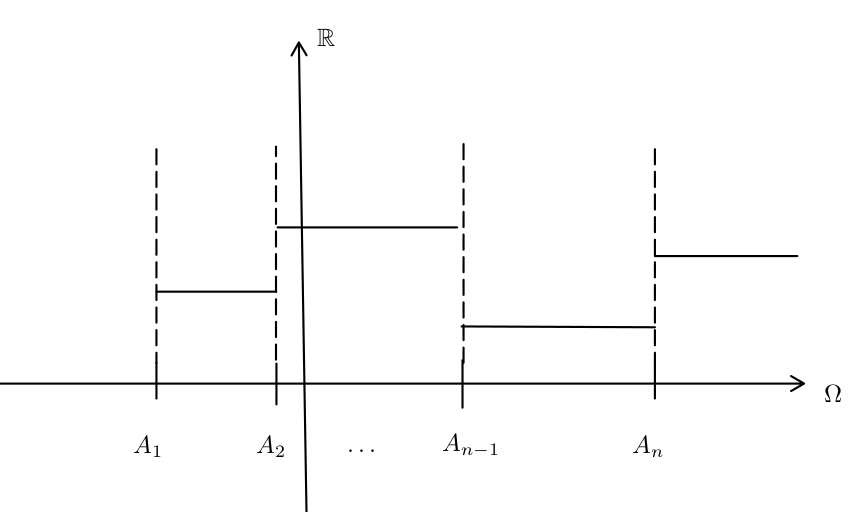
\includegraphics[scale=0.3]{figures/sigma_n.png}
  \caption{Dans ce cas, $\sigma(X) = \sigma$-algèbre engendrée par la partition $\mathscr{A}$.}
  \label{ss-x-partition}
\end{figure}

\begin{remark}[Personnelle]
  On rappelle que pour la figure \ref{ss-x-partition}, si \(A_1, \dots, A_n\) est une partition de l'ensemble \(X\), on définit

  \[
  \tau = \left\{ \bigcup _{i \in J} A_i, J \subset \{ 1, \dots, n \} \right\}.
  \]

  On démontre que $\tau$ est une tribu.
\end{remark}

\section{Indépendance de variables aléatoires}


\begin{definition}
  Deux variables aléatoires $X_1, X_2$ sont indépendantes si $\sigma(X_1) = X_1 ^{-1} (\beta )$ et $\sigma(X_2) = X_2 ^{-1} (\beta )$ sont deux \textbf{familles indépendantes} (cf définition \ref{sigma-alg-indep}).
\end{definition}

Un élément de $X ^{-1} (\beta )$ s'écrit comme $X ^{-1} (B_1), B_1 \in \beta$.

On écrira alors

\[
\mathbb{P}(X_1 ^{-1} (B_1) \cap X_2 ^{-1} (B_2)) = \mathbb{P}(X_1 ^{-1} (B_1)) \mathbb{P}(X_2 ^{-1} (B_2)).
\]

On aura par conséquent, pour $(-\infty, b]$ qui engendrent $\beta$ (\( \{ (-\infty, b] \} \) est un \(\pi\)-système),

\[\mathbb{P}(X_1 ^{-1} ((-\infty,b_1]) \cap X_2 ^{-1} (-\infty,b_2]) = \mathbb{P}(X_1 ^{-1} (-\infty,b_1]) \mathbb{P}(X_2 ^{-1} (-\infty, b_2]), \]

donc

\[\mathbb{P}(X_1 \in (-\infty, b_1], X_2 \in (-\infty, b_2]) = \mathbb{P}(X_1 \in (-\infty,b_1]) \mathbb{P}(X_2 \in (-\infty, b_2]).\]

On obtient ainsi

\begin{equation}
  \mathbb{P}(X_1 \leq b_1, X_2 \leq b_2)  = \mathbb{P}(X_1 \leq b_1) \mathbb{P}(X_2 \leq b_2). \label{indep-def}
\end{equation}


\marginpar{25-09-2023}

Le résultat \ref{indep-def} est exactement la définition de l'indépendance des deux variables aléatoires.

On peut écrire \ref{indep-def} en terme de lois de probabilités :


\begin{equation}\label{indep-loi}
  \mathbb{P}(\overbrace{X_1 \leq b_1, X_2 \leq b_2}^{\subset \Omega}) = P_X((-\infty, b_1] \times (-\infty, b_2]) \stackrel{\text{si indép}}{=} P _{X_1}((-\infty, b_1]) P _{X_2}((-\infty, b_2]).
\end{equation}


\begin{prop}
  Deux variables aléatoires \(X_1, X_2\) définies sur l'espace \((\Omega, \mathscr{A}, \mathbb{P} )\) sont indépendantes si et seulement si

  \[P _{(X_1, X_2)} = P _{X_1} P _{X_2}.\]
\end{prop}

\begin{proof}

  \

  \begin{enumerate}
    \item \emph{Partie nécessaire.} On l'a démontré dans \ref{indep-loi}.
    \item \emph{Partie suffisante.} On suppose que

    \[\overbrace{P _{(X_1, X_2)}(B_1 \times B_2)}^{\text{loi du couple}}  = P _{X_1}(B_1) P _{X_2}(X_2).\]

    On prend $B_1 =(-\infty, b_1]$ et \(B_2 = (-\infty, b_2]\).

    Ainsi

    \[P _{(X_1, X_2)}((-\infty, b_1] \times (-\infty,b_2]) = \mathbb{P}(X_1 \leq b_1, X_2 \leq b_2).\]
  \end{enumerate}
\end{proof}


\begin{exemple}
  Considérons un vecteur aléatoire \((X_1, X_2)\) de loi

  \[\begin{cases}
     P _{X_1} = \frac{1}{2} \delta _{a_1} + \frac{1}{2}\delta _{a_2} = f_1(y)dy \\
     P _{X_2} = f_2(x) dx.
  \end{cases}\]

  On veut trouver la loi de \((X_1, X_2)\).
\end{exemple}

On calcule :

\begin{gather*}
  \int_{}^{} e^{X_1+X_2} d \mathbb{P} = \iint_{} e^{x_1+x_2} d P _{(X_1, X_2)} P(x_1, x_2) = \iint e^{x_1+x_2} d\left(\frac{1}{2} \delta _{a_1} + \frac{1}{2}\delta _{a_2}\right)f_2 d x_2 = \dots
\end{gather*}

\begin{corollary}
  Si $X_1, X_2$ sont indépendantes, la même chose est vraie pour $f(X_1)$ et $g(X_2)$ avec $f$ et $g$ réelles et mesurables.
\end{corollary}

\begin{prop}
  Les variables aléatoires $X_1$ et $X_2$ sont indépendantes si et seulement si pour toutes $f, g$ non-négatives, on a

  \[\mathbb{E}[ f(X_1)g(X_2) ] = \mathbb{E}[ f(X_1) ] \mathbb{E}[ g(X_2) ]\]

  et la même chose pour $f$ et $g$ réelles et bornées.
\end{prop}

\begin{proof}

  \begin{enumerate}
    \item \emph{Partie nécessaire.}

    \begin{equation}
      \int_{\Omega}^{} f(X_1)g(X_2) d \mathbb{P} = \iint_{\mathbb{R}^2} f(x_1) g(x_2) d _{X_1 X_2} P(x_1, x_2).  \label{marg}
    \end{equation}

    Or si les variables sont indépendantes, la loi \(P _{X_1 X_2}\) se factorise dans les marginales.

    Donc \ref{marg} devient :

    \begin{gather*}
      \iint_{\mathbb{R}^2} f(x_1)g(x_2) d P_{X_1}(x_1) d P _{X_2}(x_2) = \int_{\mathbb{R}}^{} f(x_1) d P _{X_1}(x_1) \int_{\mathbb{R}}^{} g(x_2) d P _{X_2}(x_2) = \mathbb{E}[X_1] \mathbb{E}[X_2].
    \end{gather*}

    \item \emph{Partie suffisante.} On considère $f = \mathds{1}_{(-\infty, b_1]} \text{ et } g= \mathds{1}_{(-\infty,b_2]}. $

    On a

    \begin{gather*}
      \int_{}^{} \mathds{1}_{(-\infty, b_1]} \circ X_1 \mathds{1}_{(-\infty, b_2]} \circ X_2 d \mathbb{P} = \mathbb{E}[f(X_1)g(X_2)] = \mathbb{E}[f(X_1)] \mathbb{E}[g(X_2)] = \mathbb{P}(X_1 \leq b_1) \mathbb{P}(X_2 \leq b_2).
    \end{gather*}


  \end{enumerate}

\end{proof}

  \begin{prop}[Indépendance et fonctions de répartition]
    Les variables aléatoires $X_1$ et $X_2$ sont indépendantes si et seulement si

    \[F _{X_1, X_2}(t_1, t_2) = F _{X_1}(t_1) F _{X_2}(t_2).\]
  \end{prop}

  \begin{proof}
    \begin{enumerate}
      \item \emph{Partie nécessaire.} Si les variables aléatoires \(X_1, X_2\) sont indépendantes, alors

      \begin{gather*}
        F _{X_1, X_2}(t_1, t_2) = \mathbb{P}(X_1 \leq t_1, X_2 \leq t_2) = \mathbb{P}(X_1 \leq t_1) \mathbb{P}(X_2 \leq t_1) = F _{X_1}(t_1) F _{X_2}(t_2).
      \end{gather*}

      \item \emph{Partie suffisante.} Point de départ : on écrit la condition

      \[  \mathbb{P}(X_1 \leq t_1, X_2 \leq t_2) = F _{X_1 X_2}(t_1, t_2) = F _{X_1}(t_1) F _{X_2}(t_2)= \mathbb{P}(X_1 \leq t_1) \mathbb{P}(X_2 \leq t_2) ,\]

      avec \(t_1, t_2\) quelconques et on obtient que \(X_1 \text{ et } X_2 \) sont indépendantes comme c'est dit dans la définition \ref{indep-def}.
    \end{enumerate}
  \end{proof}

  \begin{prop}[Indépendance et densités]

    \

    \begin{enumerate}
      \item Soient $X_1, X_2$ deux variables aléatoires avec les densités $f _{X_1}$ et $f _{X_2}$ et supposons que \(X_1\) et \(X_2\) sont indépendantes. Alors le couple \((X_1, X_2)\) et sa densité vérifient :

      \[f _{X_1, X_2}(x_1, x_2) = f _{X_1}(x_1) f _{X_2}(x_2).\]

      \item Supposons que $(X_1, X_2)$ admet la densité $f _{X_1, X_2}(x_1, x_2)$ qui est le produit entre deux fonctions intégrables non-négatives $\tilde{f}_1(x_1), \tilde{f}_2(x_2)$. Alors $\tilde{f}_1(x_1)$ et \(\tilde{f}_2(x_2)\) sont à des facteurs multiplicatifs près, les densités de \(X_1\) et \(X_2\) sont \textbf{indépendantes}.
    \end{enumerate}

\end{prop}

%ъуъ

\begin{proof}

  \

  \begin{enumerate}
    \item Loi de \(X_1 \implies f _{X_1}(x_1) d x_1 : P _{X_1}\) et loi de \(X_2 \implies f _{X_2} (x_2) d x_2 : P _{X_2}\).

    \[f _{X_1, X_2}(x_1, x_2)dx_1dx_2 = P _{X_1 X_2} = P _{X_1} P _{X_2} = f _{X_1}(x_1) f _{X_2}(x_2) dx_1dx_2.\]

    \item On sait que

    \begin{gather*}
      f _{X_1}(x_1) = \int_{}^{} f _{X_1 X_2}(x_1, x_2) d x_2 = \tilde{f} _{X_1}(x_1) \int_{}^{} \tilde{f} _{X_2} (x_2) d x_2  \\
      f _{X_2}(x_2) = \int_{}^{} f _{X_1 X_2} (x_1, x_2) d x_1 = \tilde{f} _{X_2}(x_2) \int_{}^{} \tilde{f} _{X_1}(x_1) d x_1.
    \end{gather*}

    Ensuite,

    \begin{gather*}
      \iint_{\mathbb{R}^2} f _{X_1 X_2}(x_1, x_2) dx_1dx_2 = 1 = \iint_{\mathbb{R}^2} \tilde{f} _{X_1}(x_1) \tilde{f} _{X_2}(x_2) dx_1dx_2 = \int_{\mathbb{R}}^{} \tilde{f}(x_1) dx_1 \int_{\mathbb{R}}^{} \tilde{f}_{X_2}(x_2) dx_2.
    \end{gather*}

    On a

    \begin{gather*}
      f _{X_1}(x_1) f _{X_2}(x_2) = \tilde{f}_{X_1}(x_1) \tilde{f} _{X_2}(x_2) \underbrace{\int_{}^{} \tilde{f} _{X_2}(x_2) d x_2 \int_{}^{} \tilde{f}_{X_1} (x_1) d x_1}_{=1}.
    \end{gather*}

    En conclusion, on a

    \[ f _{X_1}(x_1) f _{X_2}(x_2) = \tilde{f} _{X_1}(x_1) \tilde{f} _{X_2}(x_2).\]

    Pour que $f _{X_1}$ et $f _{X_2}$ deviennent des densités, on pose :

    \[f _{X_1}(x_1) = \frac{\tilde{f} _{X_1}(x_1)}{\int_{}^{}f _{X_1}(x_1) d x_1 } \text{ et } f _{X_2}(x_2) = \frac{\tilde{f} _{X_2}(x_2)}{\int_{}^{}f _{X_2}(x_2) d x_2 }. \]
  \end{enumerate}
\end{proof}

%Réviser changement de variable dans \mathbb{R}^n.



\marginpar{26-09-2023}

%Programme :
%Convergence de VA
%Convergence en loi (fonction caractéristique)
%Théorèmes limites
%Vecteurs gaussiens
%(Espérances conditionnelles)

\section{Changement de variables}

On considère \((X_1, X_2)\) un vecteur aléatoire à densité \(f _{X_1 X_2}(x_1, x_2)\). On construit deux autres variables aléatoires \(U_1, U_2\) telles que

\[\begin{cases}
U_1 = g_1(X_1, X_2) \\
U_2 = g_2(X_1, X_2).
\end{cases}\]


On veut trouver la loi de \(U_1, U_2\), à savoir la densité du couple.

Soit \(h : \mathbb{R}^2 \to \mathbb{R}\) une fonction mesurable positive quelconque que l'on appelle ``fonction test''.

\begin{gather}
  \int_{\Omega} h(U_1, U_2) d \mathbb{P} = \int_{\Omega} h(g_1(X_1, X_2), g_2(X_1, X_2)) d \mathbb{P} \\
  \stackrel{\text{transfert}}{=} \iint_{\mathbb{R}^2} h (g_1(x_1, x_2), g_2(x_1, x_2)) d P _{X_1 X_2}\\
  = \iint_{\mathbb{R}^2} h(g_1(x_1, x_2), g_2(x_1, x_2)) f _{X_1, X_2} (x_1, x_2) d x_1 d x_2. \label{chva}
\end{gather}

On pose

\[\begin{cases}
u_1 = g_1 (x_1, x_2) \\
u_2 = g_2 (x_1, x_2).
\end{cases}\]

On sait que \((X_1, X_2)\) ne sont pas forcément définies sur \(\mathbb{R}^2\), mais sur un certain domaine \(A \subset \mathbb{R}^2\). On pose \(G = (g_1, g_2) : \mathbb{R}^2 \to \mathbb{R}^2\).

On doit avoir \(G ^{-1}  : \begin{cases}
  x_1 = d_1(u_1, u_2) \\
  x_2 = d_2(u_1, u_2)
\end{cases},\) donc il faut que \(G\) soit inversible. De plus, on devrait calculer la matrice jacobienne

\[J _{U_1 U_2} = \left(\begin{matrix}
  \frac{\partial d_1 }{\partial u_1 } & \frac{\partial d_1 }{\partial u_2} \\
  \frac{\partial d_2 }{\partial u_2 } & \frac{\partial d_2 }{\partial u_2}
\end{matrix}\right).\]

\ref{chva} devient :

\begin{gather*}
  \iint_{\mathbb{R}^2 \cap G(A)} h(u_1, u_2) f _{X_1 X_2} (d_1(u_1, u_2), d_2(u_1, u_2)) \lvert \operatorname{det}(J _{U_1 U_2}(u_1, u_2)) \rvert d u_1 d u_2.
\end{gather*}

Comme \(h\) est quelconque, on peut choisir \(h(x) = \mathds{1}_{\{ g \bg f \} }(x) \text{ et puis } h(x) = \mathds{1}_{\{ g \less f \} } \).

On obtient la formule de changement de variable :

\begin{thm}
  \[f _{U_1 U_2}(u_1, u_2) = f _{X_1 X_2}(d_1(u_1, u_2), d_2(u_1, u_2)) \lvert \operatorname{det} J _{U_1 U_2}(u_1, u_2) \rvert \mathds{1}_{G(A)}(u_1, u_2).\]
\end{thm}

\emph{Si on a deux variables aléatoires \(X_1 \text{ et } X_2 \), quelle est la loi de \((X_1+X_2)\) ?}

On introduit \[\begin{cases}
  U_1 = X_1 + X_2,
  U_2 = X_2
\end{cases} \implies \begin{cases}
  X_1 = U_1 - U_2 \\
  X_2 = U_2
\end{cases}.\]

De plus, \[J _{U_1 U_2} = \begin{pmatrix}
1 & -1 \\
0 & 1
\end{pmatrix}.\]

On calcule \[f _{U_1 U_2} (u_1, u_2) = f _{X_1 X_2}(u_1 - u_2, u_2)\] et on obtient \[f _{U_1}(u_1) = \int f _{U_1, U_2}(u_1, u_2) d u_2 = \int_{}^{} f _{X_1 X_2} (u_1 - u_2, u_2) d u_2 = \int_{\mathbb{R}}^{} f _{X_1}(u_1- u_2)f _{X_2}(u_2) d u_2. \]

Il s'agit du \textbf{produit de convolution}.








%%%%%%%%%%%%%%%%%%%%%%%%%%%%%%%%%%%
%%%%%%%%%%%%%%%%%%%%%%%%%%%%%%%%%%%
%%%%%%%%%%%DENOMBREMENT%%%%%%%%%%%%
%%%%%%%%%%%%%%%%%%%%%%%%%%%%%%%%%%%
%%%%%%%%%%%%%%%%%%%%%%%%%%%%%%%%%%%

\chapter{Dénombrement}

\marginpar{15-09-2023}

On a 3 objets $\{ a,b,c \} $.
\section{Dispositions sans répétition}

\begin{tabular}{|c|c|c|}
  \hline
  Eléments & Combinaisons sans ordre & Combinaisons avec ordre \\
  \hline
  1 à 1 & $\{ a \}, \{ b \}, \{ c \} $ & $\{ a \}, \{ b \}, \{ c \} $ \\
  \hline
  2 à 2 & $\{ a,b \}, \{ a,c \}, \{ b,c \} $ & $\{ a,b \}, \{ b,a \}, \{ a,c \}, \{ c,a \}, \{ b,c \}, \{ c,b \} $ \\
  \hline
  3 à 3 & $\{ a,b,c \} $ & $\{ a,b,c \}, \{ a,c,b \}, \{ b,a,c \}, \{ c,a,b \}, \{ c,b,a \}, \{ b,c,a \} $ \\
  \hline
\end{tabular}

\section{Dispositions avec répétition}

\begin{tabular}{|c|c|c|}
  \hline
  Eléments & Dispositions sans ordre & Dispositions avec ordre \\
  \hline
  1 à 1 & $\{ a \}, \{ b \}, \{ c \} $ & $\{ a \}, \{ b \}, \{ c \} $ \\
  \hline
  2 à 2 & $\{ a,a \}, \{ b,a \}, \{ b,b \}, \{ a,c \}, \{ b,c \}, \{ c,c \} $ & $ \{ a,a \}, \{ a,b \}, \{ b,a \}, \{ b,b \}, \{ a,c \}, \{ c,a \}, \{ b,c \}, \{ c,b \} \{ c,c \} $ \\
  \hline
  3 à 3 & $\{ a,a,a \}, \{ a,a,c \}, \dots $ (10 éléments) & $\{ a,a,a \}, \{ a,a,c \}, \{ a,c,a \}, \{ c,a,a \}, \dots $ ($3 ^3 = 27$ éléments) \\
  \hline

\end{tabular}

\begin{figure}[h!]
  \centering
  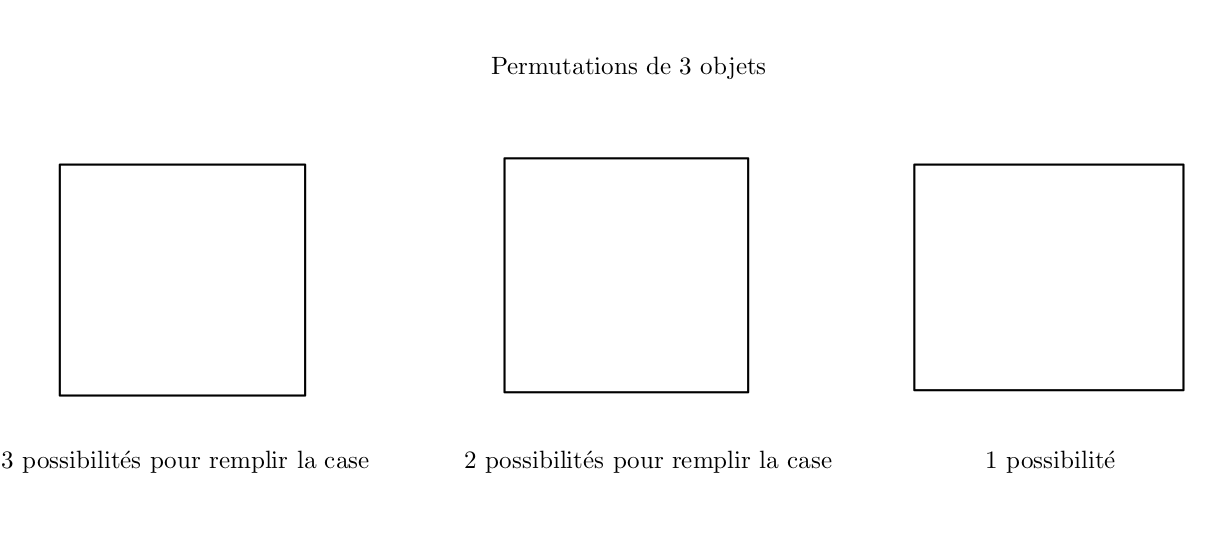
\includegraphics[scale=0.3]{figures/perm3.png}
  \caption{Permutations dans le cas de 3 objets (dispositions sans répétition et avec ordre)}
  \label{}
\end{figure}

\paragraph{Arrangements de $n$ objets pris $k$ à $k$ (dispositions avec ordre et sans répétition)} %(dans notre cas 3 objets pris 2 à 2)

Si on a 4 objets pris 2 à 2 : $\{ a,b,c,d \} $.

Si $a$ et $b$ sont fixés, alors $\{ a,b \} $ engendrera $\{ a,b,c,d \} $ et $\{ a,b,d,c \} $.

On a $$A _{n} ^{k} = \frac{n!}{(n-k)!}$$

\paragraph{Combinaisons de $n$ objets pris $k$ à $k$ (dispositions sans ordre et sans répétition)}

\begin{equation}
  C _{n} ^{k} = \frac{n!}{k!(n-k)!} = \binom{n}{k}.
\end{equation}

En fait,
\begin{equation*}
  C _{n} ^{k} = \frac{A _{n} ^{k}}{k!},
\end{equation*}

avec $k!$ le nombre de permutations des $k$ éléments.

%\paragraph{(combinaisons avec ordre et avec répétition)}

%\paragraph{(combinaisons sans ordre et avec répétition)}

Si on a $n$ objets à combiner $k$ à $k$ avec répétition, mais sans ordre, il y a

\begin{equation}
  C _{k} ^{n+1-k} = \frac{(n+1-k)!}{k!(n-1)!} \text{ combinaisons possibles.}
\end{equation}


%\begin{exo}
%  Dans une bibliothèque, il y a $n$ livres sur une étagère repartis au hasard. Parmi ces $n$ livres, $k$ sont d'un même auteur $A$, les autres d'auteurs différents. Calculer la probabilité qu'au moins $p$ livres de $A$ se retrouvent côte à côte dans les cas suivants :
%  \begin{enumerate}
%    \item $n=20, k=3, p=3$ ;
%    \item $n=20, k=5, p=2$ (\textbf{au moins} 2 livres).
%  \end{enumerate}
%\end{exo}


\section{Tirage des urnes sans remise}

$N$ boules de type $N_a, N_b$ tels que $N_a + N_b = N$.

On tire $n \less N$ boules.

Soit $E$ l'événement suivant : $\{ k \text{ boules parmi } n \text{ sont de type } a \}$.

Calculer la probabilité de $E$.

\begin{gather*}
  \mathbb{P}( E ) = \frac{C _{N_a} ^{k} C _{N_b} ^{n-k}}{C_N ^{n}} \text{ (formule hypergéométrique).}
\end{gather*}

\begin{proof}
  $\Omega = \text{ combinaisons de } N \text{ objets pris } n \text{ à } n \text{ sans les répéter. }   $

  On a $\sharp(\Omega) = C_N ^{n}$.

  Cas favorables : $C _{N_a} ^{k} C _{N_b}^{n-k}$.
\end{proof}

Cette formule est utilisée pour calculer la probabilité de gagner au loto. On a une grille de 49 numéros et on tire 6 numéros.

$N_a =$ les 6 numéros cochés par le joueur, $N_b = 49-6 = 43$ et $n=N_a$.

\begin{gather*}
  \mathbb{P}( \text{avoir 3 numéros gagnants} ) = \frac{C^{3}_{6} C^{3}_{43}}{C^{6}_{49}} \approx 0.018 \\
  \mathbb{P}( \text{avoir 6 numéros gagnants} ) = \frac{C^{6}_{6} C^{0}_{43}}{C_{49}^{6}} \approx 7,15 \times 10 ^{-8}.
\end{gather*}

\section{Tirage des urnes avec remise}

$N$ boules, $N_a$ de type $a$, $N_b$ de type $b$. On en tire $n$ (avec $n$ quelconque) et

\begin{equation*}
  E = \{ k \text{ boules parmi les } n \text{ tirées sont de type } a  \}.
\end{equation*}

On a $\sharp(\Omega) = N ^{n}$.

Cas favorables : $N_a ^{k} N_b ^{n-k} \binom{n}{k}$.

Donc

\begin{equation*}
  \mathbb{P}( E ) = \frac{N_a ^{k} N_b ^{n-k} \binom{n}{k}}{N ^{n}} = \frac{N_a ^{k} N_b ^{n-k} \binom{n}{k}}{N ^{k} N ^{n-k}} = \left( \frac{N_a ^{k}}{N}\right) ^{k} \left( \frac{N_b}{N}\right) ^{n-k} \binom{n}{k} = p_a ^{k} p_b ^{n-k} \binom{n}{k},
\end{equation*}

où $p_a$ et $p_b$ sont les pourcentages de $a$ et de $b$.

Il s'agit de la \textbf{loi binomiale}.

%%%%%%%%%%%%%%%%%%%%%%%%%%%%%%%%%%%%%%%%%%%%%%%%%%%%%%%%%%%%%%%%%%%%%%%%%%%%%%%%%%%%%%%%%%%%%%%%%%%%%%%%%%%%

\chapter{Travaux dirigés}

\begin{exo}
  Dans une bibliothèque, il y a $n$ livres sur une étagère repartis au hasard. Parmi ces $n$ livres, $k$ sont d'un même auteur $A$, les autres d'auteurs différents. Calculer la probabilité qu'au moins $p$ livres de $A$ se retrouvent côte à côte dans les cas suivants :
  \begin{enumerate}
    \item $n=20, k=3, p=3$ ;
    \item $n=20, k=5, p=2$ (\textbf{au moins} 2 livres).
  \end{enumerate}
\end{exo}

\begin{proof}

  \

  \begin{enumerate}
    \item

    \begin{figure}[h!]
      \centering
      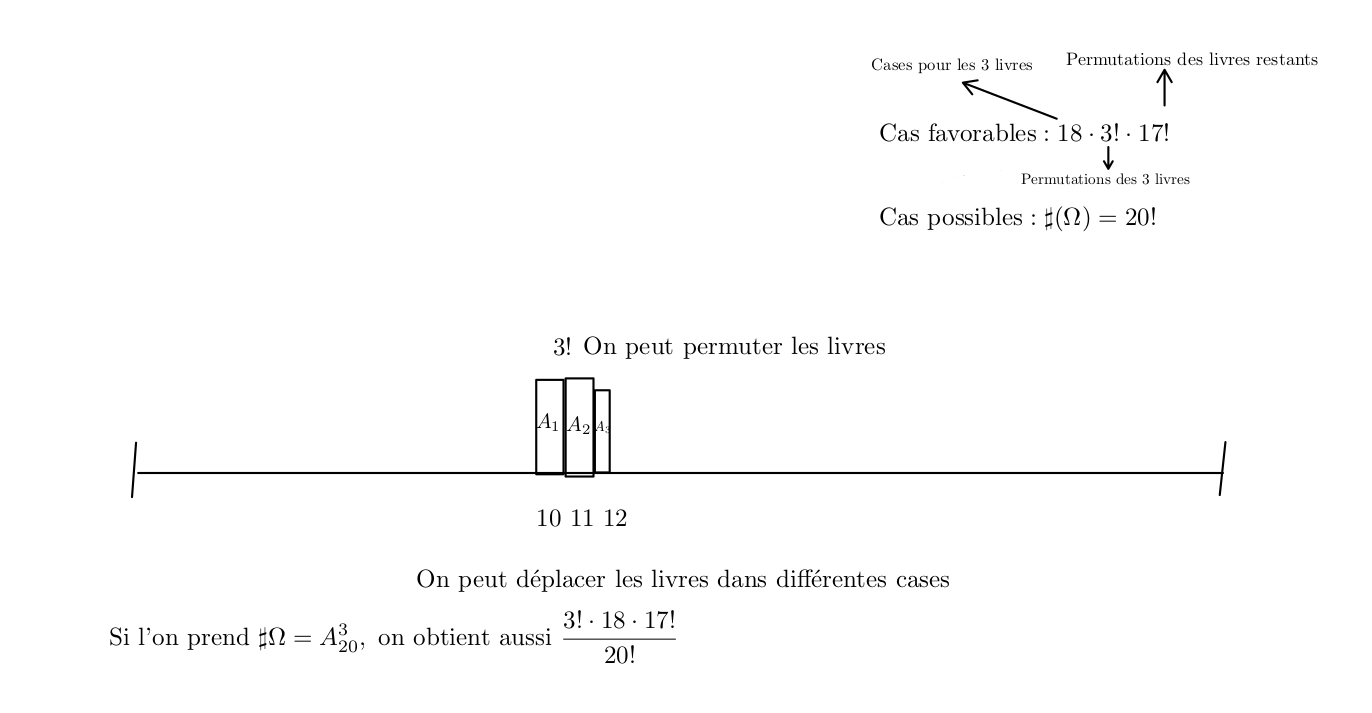
\includegraphics[scale=0.3]{figures/exo_livres.png}
      \caption{Solution pour (1)}
      \label{}
    \end{figure}

    %\item On note $E$ l'événement ``au moins 2 livres se trouvent côte à côte''. Notons $E ^{C}$ = ``il n'y a pas de livres de $A$ côte à côte''.
  \end{enumerate}
\end{proof}

\begin{exo}
  On lance 10 fois une pièce de monnaie. Calculer la probabilité qu'au cinquième lancer on obtient pile en sachant que le nombre total des piles obtenus est 3.
\end{exo}

\begin{exo}
  On a deux variables aléatoires \(X_1\) et \(X_2\) de même densité \(f(x) = \frac{1}{X ^2} \mathds{1}_{[1, \infty)}(x)\) et elles sont indépendantes. On pose
  \begin{gather*}
    U = X_1 X_2 \\
    V = \frac{X_1}{X_2}.
  \end{gather*}

  \begin{enumerate}
    \item Calculer la loi du couple \((U,V)\).
    \item \(U \text{ et } V \) sont-elles indépendantes ?
  \end{enumerate}
\end{exo}

\begin{exo}
  On place six boules de manière aléatoire et indépendante dans 3 boîtes. Calculer la probabilité que la première boîte contienne deux boules.
\end{exo}

\begin{exo}
  Un robinet a été installé le jour \(J\) et il fuit, les fuites se produisent chaque heure de manière indépendante et avec la probabilité \(p\).

  \begin{enumerate}
    \item Calculer la loi de la variable aléatoire \(F\) égale au nombre de fuites qui se sont produites tout au long de la journée (en 24 heures), ie \(\mathbb{P}(F=k), k \in \{ 0, \dots, 24 \}\).
    \item On dénote \(T(1)\) la variable aléatoire égale à l'heure de la première fuite. Calculer la loi de \(T(1)\), ie \(\mathbb{P}(T(1) = k), k=1, \dots, 24\).
    \item On dénote \(T(2)\) la variable aléatoire égale à l'heure de la deuxième fuite. Montrer que \(T(1)\) et \(T(2)-T(1)\) sont indépendantes et ont la même loi.
  \end{enumerate}
\end{exo}





\end{document}
